\documentclass[thesis]{thesis-gwu}[2020/02/03]


 
\usepackage{lipsum}
\usepackage{graphicx}
\usepackage{float}
\usepackage{booktabs}
\usepackage{adjustbox}
\usepackage{tikz}
\usepackage{comment}
%This is to centalize all the table caption. added new
\usepackage[justification=centering]{caption}





\usepackage{tikz}
\usetikzlibrary{shapes.geometric, arrows.meta, positioning}
\tikzstyle{process} = [rectangle, rounded corners, minimum width=5.5cm, minimum height=1.2cm,text centered, draw=black, fill=blue!10]
\tikzstyle{arrow} = [thick,->,>=stealth]








 
\newcolumntype{Y}{>{\centering\arraybackslash}X}




%added by me to disable doublespacing in appendix
\usepackage{setspace}

%to get rid of red keyword

%if I want to play with the color
% \hypersetup{
%   colorlinks=true,
%   linkcolor=blue, % This sets the color of internal links to blue.
%   filecolor=magenta, % Color for URLs which open local files.
%   urlcolor=blue, % Color for linked URLs.
%   citecolor=blue, % Color for bibliographic citations in text.
% }

\usepackage{hyperref} \hypersetup{ colorlinks=true, linkcolor=, filecolor=magenta,
urlcolor=blue, citecolor=blue }


% control table better. caption etc

\usepackage{caption} % For caption customization
\captionsetup[table]{justification=justified,singlelinecheck=false} % Align captions to left
\captionsetup[table]{font=it} % Makes table captions italic

  


% remove red box around TOC and reference
\hypersetup{pdfborder=0 0 0}

%my import added by me
 
% to include source code
\usepackage{xcolor} 
\usepackage{listings}
\renewcommand{\lstlistingname}{Source Code}
\renewcommand{\lstlistlistingname}{Source Code}

\usepackage{color}
\definecolor{codegreen}{rgb}{0,0.6,0}
\definecolor{codegray}{rgb}{0.5,0.5,0.5}
\definecolor{codepurple}{rgb}{0.58,0,0.82}
\definecolor{backcolour}{rgb}{0.95,0.95,0.92}

\lstset{
language=Python,
backgroundcolor=\color{backcolour},
commentstyle=\color{codegreen},
keywordstyle=\color{magenta},
numberstyle=\tiny\color{codegray},
stringstyle=\color{codepurple},
%basicstyle=\ttfamily\small,
basicstyle=\fontsize{8}{9}\selectfont\ttfamily,
breakatwhitespace=false,         
breaklines=true,                 
captionpos=b,                    
keepspaces=true,                 
numbers=left,                    
numbersep=5pt,                  
showspaces=false,                
showstringspaces=false,
showtabs=false,                  
tabsize=2,
frame=single,
rulecolor=\color{black},
title=\lstname
}

 


% by me
\usepackage{tabularx} % Allows for tables that stretch to fit a given width

%for testing beautiful tables

%me for better table normal size font

\usepackage{tabularx} % For tables that automatically adjust their width
\usepackage{makecell} % Allows for line breaks within table cells
 
 
% include pdf
\usepackage{pdfpages}

 
%using this to add caption to my included pdf in the appendix
\usepackage{caption}
 
 

%color table
\usepackage{colortbl}

%table multirow
\usepackage{multirow} 
 
%\usepackage{subfigure}
\usepackage[style=apa, backend=biber]{biblatex}
%\usepackage[style=apa,backend=biber,language=american]{biblatex}
%\DeclareLanguageMapping{american}{american-apa}

%\usepackage{natbib}



%\addbibresource{thesis-bib.bib}
\addbibresource{mybib.bib}


% !TEX root = ../thesis-sample.tex

% --------- FRONT MATTER PAGES ---------------------

% Title of the thesis
\title{Your Praxis Tile. First letter of every word is capitalized}
% capitalize significant words!

% Author name
\author{Your Name}

% Previous degrees
\bachelordegree{Bachelor of Science}
\bsdepartment{Your Major}
\bsschool{your University }
\bsgrad{month year} % "month year"

\masterdegree{M.S.}
\msdepartment{Your Major}
\msschool{your University }
\msgrad{August 2014}  % "month year"
% you can show or hide the MS degree line
\showmsdegree
% \hidemsdegree

% PhD degree commands
% Committee
\showcommitteepage % hide this page if you're doing a MS thesis
%\hidecommitteepage 


% define COMMITTEE information

% in general, note that administrative titles are not used, instead use "professorial titles"?

% Chair must be entered separately for formatting reasons.
\chair{[Your Advisor Name]}
%\department{Professorial Lecturer in Engineering and Applied Science}
\chairtitle{Professorial Lecturer in  Engineering and Applied Science}

% uncomment and use the below if you have a co-chair. note the code reacts to the \cochair{} , not the \cochairtitle{}
% \cochair{Co-Chair Person}
% \cochairtitle{Just-as-Amazing Professor of \insertdepartment}

\phdschool{The School of Engineering and Applied Science}

\committee{ 
% director first
\insertchair, \insertchairtitle, Praxis Director

% remember to add a space between committee members
%\vspace{\baselineskip}

\IfNoText{\insertcochair}
    { % if you have no co-chair, leave \cochair{} undefined/blank and fill in the next line
    % Full Name, Title, Praxis Director/Praxis Co-Director/Committee Member \hfill
    % Shahryar Sarkani, Professorial Lecturer of Engineering and Applied Science, Committee Member \hfill

    }{ % if you have defind these, it will fill in the below:
        \insertcochair, 
        \IfNoText{\insertcochairtitle}{\textbf{DEFINE CO-CHAIR TITLE}}{\insertcochairtitle}, 
        Praxis Co-Director \hfill
    }

%\vspace{\baselineskip}

% note you shouldn't write "The George Washington University" at all- it is implied
% Full Name, Title, Praxis Director/Praxis Co-Director/Committee Member \hfill
% Shahryar Sarkani, Professorial Lecturer of Engineering and Applied Science /Committee Member \hfill

\vspace{\baselineskip}

XYZ, Professor of Online Engineering Programs, Chair \hfill

\vspace{\baselineskip}

XYZ, Professorial Lecturer of Engineering and Applied Science, Committee Member \hfill


% external examiner
% Name of External Examiner, Professorial Title, Name of External University (or Name, Job Title, Name of External Company), Committee Member  % include university or company of any external examiner! but still "committee member"
}

\phdgrad{Month DD, 2025}  % Month DD, YYYY
\defensedate{Month DD, 2025}  % Month DD, YYYY
% Year of completion for copyright page and perhaps other places
\year=2025

% Copyright page
%\copyrightholder{Someone else}

% Dedication
\dedication{ %
\emph{
\lipsum[1]
}
}

% Acknowledgments
\acknowledgments{
\lipsum[1]

}



% commands to show or hide front matter pages
% ############################THIS I CHANGE TO SHOW AND HIDE#########
\showcopyright
\showabstract
\showcommitteepage
\showdedication
\showacknowledgments
\hidepreface
\hideprologue
\hideforeword

% Commands to hide or show lists of figures, tables, etc.
\showtableofcontents
\showlistoffigures
\showlistoftables
\hidenomenclature
%###################################################THE ABOVE IS WHAT WAS WORKING






% ^ NOTE! April 4 hack for April 15 deadline - if any of these are missing from your TOC and there should be entries there, see lines 1435-1447 of the class file for an example. You need to wrap the appropriate function call adding a call to addcontentsline





 

 
% call an abbreviation using \ac{abbrev}

% symbols and acronyms only show up when used in the text
% \symbols{
%     \acro{J}{Moment of Inertia}
% }       

% if you want acronym (simpler) then change these to show
% hiding this usinbg hide instead of show removed the first emtpy list of abbreviation page, but to show the list of abbreviation you need to use showglossarieslistofabbreviations so it will be listed as part of glossariies


\hidelistofabbreviations
% I changed this from show to hide this and also the showglossarieslistofsymbols  to hide and that indeed hid the list of symbol page
\hidelistofsymbols

% if you want glossaries (more powerful) then leave above as hide
% GLOSSARIES package options - automatically turns off front pages from acronym package

% acronymns and symbols are basically the same, but there are two provided 
% locations where they can show up

% these three were not hidden original. I hid them (all three below)
%\setabbreviationstyle[acronym]{long-short}
%\setabbreviationstyle[abbreviation]{long-short}
\makeglossaries



% you can hide/show the glossaries page


\hideglossarieslistofabbreviations
\hideglossarieslistofsymbols
\showglossariesglossaryofterms


%####################################################################
%##
%##   You need to add all of your Glossaries one at a time.  ########
%##
%######################################################################

 



\newglossaryentry{AI}{name=AI, description={Artificial Intelligence}}
\newglossaryentry{ANN}{name=ANN, description={Artificial Neural Network}}
\newglossaryentry{API}{name=API, description={Application Programming Interface}}

\newglossaryentry{SHAP}{name=SHAP, description={SHapley Additive exPlanations}}

\newglossaryentry{SVM}{name=SVM, description={Support Vector Machine}}
\newglossaryentry{TN}{name=TN, description={True Negative}}
\newglossaryentry{TP}{name=TP, description={True Positive}}
\newglossaryentry{UBB}{name=UBB, description={User-Based Batching}}
\newglossaryentry{UBS}{name=UBS, description={User-Based Sequencing}}



\abstract{
\lipsum[1]
 
 

}

% This is by me. It will add abbreviation , list of sybolsm Glossary of terms
% I found out I don't need the next two lines as they will also print the abbrev and symbols
% in the front of the page
% \glsaddall
% \printglossaries
\glsaddallunused 

%The above glsaddallunused made the glossary appear

%% DOCUMENT AREA

\begin{document}
\chapter{Introduction}
\section{Background}


\lipsum[1]. 

\textcolor{red} {This is how you insert a citation to the references you added in your mybib.bib file. \parencite{chung2014empirical}. And this is in text citation \textcite{du2017deeplog} said so and so...Please note the references will be added automatically to your reference section in the correct format as defined by the template}. Please remove the color. 


\section{Problem in the area of research}
\lipsum[1]

\section{Research Motivation}
 
\lipsum[1]

\section{Problem Statement}
\textcolor{red}{\textit{\textit{A sharp rise in  ... threats has exposed ... to increasing data breaches (Gurucul, 2023), Costing ... per breach \parencite{IBM2023CostDataBreach}.}}}\par

\textcolor{blue}{Please note:} Include your problem statement exactly as it is and italicize it. The problem statement should stand alone as a single paragraph. You can elaborate on it in the rest of the section. Make sure to remove any text coloring.
 
\lipsum[1]


\section{Thesis Statement}
\textcolor{red}{\\textit{\textit{A predictive model using XYZ and XYZ2 will efficiently xxxxxxx.}}}\par

\textcolor{blue}{Please note:} The same applies to the Thesis Statement. Include it verbatim as a single paragraph. You may expand on it in a subsequent paragraph. Ensure all text coloring is removed.
 
\lipsum[1]

\section{Research Objectives}
 
\lipsum[1]

\section{Research Questions and Hypotheses}


\lipsum[1] \par 

\textcolor{red}{Here, you will put your research question and hypothesis exactly as you had them in your proposal document. You will use RQ1: followed by the question and then a new line, and then the second question, newline, the third question, then newline the hypotheses. Each in a line by itself. Please remove the coloring.}


\textbf{RQ1:} Your question1 1 xxxx.?\par

\textbf{RQ2:} Your question1 1 xxxx.\par

\textbf{RQ3:} Your question1 1 xxxx.\par

\textbf{H1:} Your hypothesis 1 xxxx.\par

\textbf{H2:} Your hypothesis 2 xxxx. \par

\textbf{H3:} Your hypothesis 3 xxxx.\par

\section{Scope of Research}
 
\lipsum[1] \par 

\section{Research Limitations}
 
\lipsum[1] \par 

\section{ Organization of Praxis}

\lipsum[1] \par   
\chapter{Literature Review}
\section{Introduction}


% we need this in the preamble

% \usepackage{tikz}
% \usetikzlibrary{shapes.geometric, arrows.meta, positioning}
% \tikzstyle{process} = [rectangle, rounded corners, minimum width=5.5cm, minimum height=1.2cm,text centered, draw=black, fill=blue!10]
% \tikzstyle{arrow} = [thick,->,>=stealth]



 


\lipsum[1]


\section{Some Section}

\lipsum[1] 

\textcolor{red}{This is how you insert an image by referencing it like this:} Figure \ref{fig:encoder-only} shows XYZ.
 

\begin{figure}[H]
    \centering
    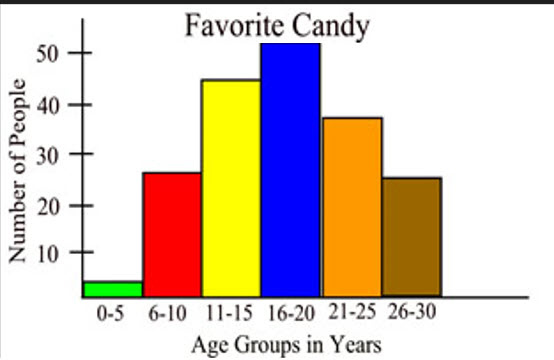
\includegraphics[width=0.6\textwidth]{figures/chap2_fig/histogram1.jpg}
    \captionsetup{
    labelfont={bf,it}, 
    textfont=it,  
    }
    \caption{Histogram of XYZ}
    \label{fig:encoder-only}
\end{figure}

\lipsum[1]

\subsection{Subsection 1}
\lipsum[1]
 
\textcolor{red}{This is how to enter an equation and reference it. Equation \ref{eqn:pos1} and \ref{eqn:pos1} show how XYZ is implemented.
}

\begin{equation}
\label{eqn:pos1}
    TE_{(pos,2i)}=sin(pos/23^{2i/Lm})
\end{equation}

\begin{equation}
\label{eqn:pos2}
    KN_{(pos,2i+1)}=cos(pos/453^{2i/Lm})
\end{equation}
 
\lipsum[1]

  

\section{Another Section}

 
\lipsum[1]

\textcolor{red}{This is the correct format for a table, including the caption and proper alignment (centered and italicized).}

\begin{table}[H]
\centering
\captionsetup{
    labelfont=bf, 
    textfont=it,  
    justification=centering
}
\caption{My Table About Something}
\label{tab:sampling-techniques}
\begin{tabularx}{\textwidth}{@{}X X@{}}
\toprule
\rowcolor[gray]{0.95} % Lighter shade for subtlety
\textbf{Reference} & \textbf{Technique} \\
\midrule
something here & Technique here \\
something here & Technique here\\
something here  & Technique here \\
something here  & Technique here\\
something here  & Technique here \\
\bottomrule
\end{tabularx}
\end{table}
 

\subsection{Subsection}
 
\lipsum[1]
 
\subsection{Subsection}
\lipsum[1]
 
 
\subsubsection{Sub subsection}
 
\lipsum[1]

 
 
\section{Summary}

\lipsum[1]  
\chapter{Methodology}
\section{Introduction}
\lipsum[1]


\section{Some Subsection}
\lipsum[1]



\section{Some Subsection}
\lipsum[1]

\subsection{Some Subsection}
\lipsum[1]



\subsection{Some Subsection}
\lipsum[1]

 
\section{Conclusion}
\lipsum[1]

 
\textcolor{red}{At the end of Chapter 3, you must restate your research questions and hypotheses exactly as they are. The format should follow the structure shown below. Please Ensure all text coloring is removed.:}\par
RQ1:\par
RQ2:\par
RQ3:\par
H1:\par
H2:\par
H3:\par
 
 

Example:

This methodological approach addresses the research questions and hypotheses outlined in Chapter 1 and repeated below:


\textbf{RQ1:} You will repeat your research question1 here?\par

\textbf{RQ2:} You will repeat your research question2 here?\par

\textbf{RQ3:} \textbf{RQ2:} You will repeat your research question3 here?\par\par

\textbf{H1:} \textbf{RQ2:} You will repeat your research Hyothesis1 here.\par

\textbf{H2:} You will repeat your research Hyothesis2 here.\par

\textbf{H3:} You will repeat your research Hyothesis2 here.\par



 
\chapter{Results and Analysis}
\section{Introduction}
\lipsum[1]
 
\section{Some Subsection}
 
\lipsum[1]
\section{Some Subsection}
\lipsum[1]

\textcolor{red}{This is how you build and format the table. The caption is centered and italized and in the top. The table number is bolded. Please remove the red coloring i use to illutrate this.}

Table \ref{tab:stat_summary} presents an overview of xyz  and zkm and xyz xyz. Lorem ipsum dolor sit amet, consectetuer adipiscing elit. Ut purus elit,vestibulum ut, placerat ac, adipiscing vitae, felis. Curabitur dictum gravida mauris. Nam arcu libero, nonummy eget, consectetuer id, vulputate a,
magna. Donec vehicula augue eu neque. Pellentesque habitant morbi
tristique senectus et netus et malesuada fames ac turpis egestas. Mauris

 

\begin{table}[H]
\centering
\captionsetup{
    labelfont={bf,it}, 
    textfont=it,  
    justification=centering
}
\caption{Title of the table every first letter capitalized}
\label{tab:stat_summary}
\begin{tabular}{lrr}
\toprule
Factor1                                      & \multicolumn{1}{c}{Test 1} & \multicolumn{1}{c}{Test 2}   \\
\midrule
Something here    & 123         & 123    \\
Something here    & 123          & 123   \\
Something here    & 123          & 1123  \\
Something here    & 16          & 123    \\
Something here    & 123        & 123     \\
Something here    & 123        & 123    \\
       \\
\bottomrule
\end{tabular}
\end{table}

\lipsum[1]

\section{Some Subsection}

 
\lipsum[1]

\textcolor{red}{This is the correct way to add and format an equation. Ensure the formatting is consistent, and remove any red coloring used for illustration.}

\begin{equation}
Accuracy = \frac {TP+TN}  {TP+TN+FP+FN}
\end{equation}

\lipsum[1].  

\textcolor{red}{This is the correct way to add and format an equation. Ensure the formatting is consistent, and remove any red coloring used for illustration.}

\begin{equation}
Precision = \frac{TP}{TP+FP}
\end{equation}
 
 
\section{Some Subsection}

\lipsum[1] 

\textcolor{red}{This is the correct way to build and format a table. The caption should be centered, italicized, and placed at the top. The table number should be bolded. In this example, the table is long, so ensure the table font matches the font of your document. It is not allowed to significantly reduce the table font size just to make it fit. In this case, I used a slightly smaller font, depending on the situation—only if necessary. However, try to avoid having too many columns to maintain readability. Make sure to remove the red coloring used for illustration.}

Table \ref{tab:xyz1} depicts the xxxx.


 


\begin{table}[H]
\centering
\captionsetup{
    labelfont={bf,it}, 
    textfont=it, 
    justification=centering
}
\caption{Test-2: Transformer vs. AutoTAB Performance Metrics}
\label{tab:xyz1}
%{\scriptsize % Applying smaller font size
{\footnotesize 
\begin{tabular}{lllllllll}
\toprule
\rowcolor[HTML]{E8F4FC} 
\textbf{Model} & \textbf{\shortstack{Method}} & \textbf{A} & \textbf{P} & \textbf{R} & \textbf{F1} & \textbf{AUC} & \textbf{FNR} & \textbf{FPR} \\
\midrule
\multirow{3}{*}{Mod1} & Sub1    & \textbf{0.0123} & \textbf{0.0123} & \textbf{0.0123} & \textbf{0.0123} & \textbf{0.0123} & \textbf{0.0123} & \textbf{0.0123} \\
                             & Sub2      & 0.0123          & 0.0123          & 0.0123          & 0.0123         & 0.0123          & 0.0123         & 0.0123 \\
                             & Sub3  & 0.0123          & 0.0123         & 0.0123          & 0.0123          & 0.0123          & 0.0123          & 0.0123 \\
\midrule
\multirow{3}{*}{Mod2}     & Sun1   & 0.0123          & 0.0123          & 0.0123          & 0.0123          & 0.0123          & 0.0123          & 0.0123 \\
                             & Sub2      & 0.0123          & 0.0123          & 0.0123          & 0.0123          & 0.0123         & 0.0123          & 0.0123 \\
                             & Sub3  & 0.0123          & 0.0123          & 0.0123         & 0.0123          & 0.0123          & 0.0123          & 0.0123 \\
\bottomrule
\end{tabular}
} % End of scriptsize scope
\end{table}



\subsubsection{Sub Subsection}

\lipsum[1]

\subsection{Subsection}
\lipsum[1] 

\section{Some Section}
\lipsum[1] 

\lipsum[1] 
\subsection{ Conclusion}
\lipsum[1] 

\textcolor{red}{
At the end of Chapter 3, you must restate your research questions and hypotheses exactly as they are. The format should follow the structure shown below. Please Ensure all text coloring is removed.:}\par
RQ1:\par
RQ2:\par
RQ3:\par
H1:\par
H2:\par
H3:\par


 

Example:

The results from this Chapter address the research questions and hypotheses outlined in Chapter 1 and repeated below:


\textbf{RQ1:} How do Transformer encoders compare to Autoencoders in terms of accuracy, precision, and recall when detecting malicious insider threats?\par

\textbf{RQ1:} You will repeat your research question1 here?\par

\textbf{RQ2:} You will repeat your research question2 here?\par

\textbf{RQ3:} \textbf{RQ2:} You will repeat your research question3 here?\par\par

\textbf{H1:} \textbf{RQ2:} You will repeat your research Hyothesis1 here.\par

\textbf{H2:} You will repeat your research Hyothesis2 here.\par

\textbf{H3:} You will repeat your research Hyothesis2 here.\par



 
\chapter{Discussion and Conclusions}
 

\section{Conclusion}
\lipsum[1]

\section{Contribution to the Body of Knowledge}
\lipsum[1]


\section{Recommendations for Future Research}
\lipsum[1]

  
%\include{tex/results-example.tex}

 

\printbibliography[title=References]

 


\include{tex/appendix-ex}

% if you want to enable appendix uncomment the line below. Alsi you need to create your appendix file  in tex/appendix-ex

%\appendix
 

\end{document}